\section{Translation and Ribosomal Synthesis as a Rate-Limiting Step}
Having now completed our circuit through key processes of cellular growth,
we find that on the whole our estimates have been reasonably successful in predicting
the scale of absolute protein copy number as well as the observed dependence on
the growth rate. This suggests that cells modulate their proteomic
composition and absolute protein abundance to better match their growth rate
requirements, without any one process representing a particular bottleneck. In
our effort to identify key limitations on growth, however, there are two notable
observations that we highlight here. The first is a recurring theme throughout
our estimates, which is that any inherent biochemical rate limitation can be
overcome by expressing more proteins. We can view this as a parallelization of
each biosynthesis task, and helps explain why bacteria
tend to increase their protein content (and cell size) as they grow faster
\citep{ojkic2019}. The second is that the synthesis of ribosomal proteins presents a
special case where parallelization is not possible (\FIG{ribosome_limit}(A)),
suggesting the possibility that it may represent a rate-limiting step in
maximizing growth rate. In the remaining sections we show how ribosome synthesis
indeed limits the acheivable growth rate, and we consider how \textit{E. coli}
deals with this constraint through control its ribosome copy number and
proteomic composition.  We then propose a minimal model of growth rate control and use this
to gain insight into how the observed changes in proteomic composition and absolute
abundance enable cells to better optimize their growth rate across different
nutrient conditions.

% \subsection{Translation and Ribosomal Synthesis as a Rate-Limiting Step}
%Thus far, the general back-of-the-envelope estimates have been reasonably
%successful in predicting the scale of absolute protein copy number as well as
%their observed dependence on the cellular growth rate. A recurring theme across
%these varied biological processes is the ability of cells to  parallelize tasks
%through the expression of additional proteins.  Even when that is not possible,
%like in chromosomal replication which  requires a minimum of $\approx$ 40
%minutes, \textit{E. coli} and many other bacteria surpass this limit by
%initiating additional rounds of replication per doubling as we have noted. However, the synthesis
%of ribosomal proteins presents a special case where parallelization is not
%possible and must be doubled in quantity on average with every cell division
%(\FIG{ribosome_limit}(A)).

\subsection{Maximum Growth Rate is Determined by the Ribosomal Mass Fraction}
To gain some intuition into how ribosomes influence
bacterial growth, we again consider the total number of peptide bonds that must
be synthesized, which we denote as $N_\text{pep}$. With cells growing exponentially in time
\citep{godin2010}, the rate of cellular growth will be related to the rate of protein synthesis by
\begin{equation}
    N_\text{pep} \lambda = r_t R f_a,
    \label{eq:mass_balance}
\end{equation}
where $\lambda$ is the cell growth rate in s$^{-1}$, $r_t$ is the maximum
elongation rate in AA$\cdot$s$^{-1}$, and $R$ is the average ribosome copy
number per cell. The addition factor $f_a$ refers to the fraction of actively
translating ribosomes, and allows us to account for the possibility of
nonfunctional, immature ribosomes or active sequestration of ribosomes, mediated
by the secondary-messenger molecule alarmones, guanosine pentaphosphate
[(p)ppGpp] at slow growth \citep{dennis2004, dai2016}.
% Knowing the number of
% peptide bonds formed per cell permits us to compute the translation-limited growth
% rate as
% \begin{equation}
% \lambda_\text{translation-limited} = \frac{r_t R f_a}{N_\text{pep}}.
% \label{eq:lambda_limit}
% \end{equation}

Alternatively, since we are most interested in the role of ribsomal synthesis on
growth rate, we instead consider this in terms of the ribosomal mass fraction, denoted by $\Phi_R$. $N_\text{pep}$ is related to the total protein mass
through the molecular weight of each protein, we can also consider the growth
rate in terms of the fraction of the total proteome mass dedicated to ribosomal
proteins. By making the approximation that an average amino acid has a molecular
weight of 110 Da (BNID: 104877), the total protein mass $m_\text{protein}$ is
related to $N_\text{pep}$ by $(m_\text{protein}/\text{110 Da}) \times N_A$,
where $N_A$ is Avogadro's number. Similarly, $R$ is related to the ribosomal
protein mass by $R \approx (m_R/\text{800 Da}) \times N_A$, where 800 Da
reflects the summed molecular weight of all ribosomal subunits.  This allows us
to approximate  $R / N_\text{pep} \approx \Phi_R / L_R$,  where $\Phi_R$ is the
ribosomal mass fraction $m_\text{protein}/m_R$, and $L_R$ the ratio of 800 kDa /
110 Da per amino acid or, alternatively, the total length in amino acids that
make up a ribosome. The translation-limited growth rate can then be written in
the form
\begin{equation}
\lambda_{\textrm{translation-limited}} \approx \frac{r_t}{L_R}  \Phi_R f_a.
\label{eq:translation_limit_growth_rate}
\end{equation}
This is plotted as a function of the ribosomal fraction $\Phi_R$ in
\FIG{ribosome_limit}(B), where we take $L_R \approx$ 7500 AA, corresponding to
the length in amino acids for all ribosomal subunits of the 50S and 30S complex
(BNID: 101175), and $f_a$ = 1. To allow us to consider the the proteomic data,
we use recent measurements of $f_a$ from \cite{dai2016} to estimate the active
fraction of ribosomal protein across each proteomic data set
(\FIG{ribosome_limit}(C)). We find that cells in general appear to
skirt this limit in growth rate as nutrient conditions vary. There is a notable discrepency
in the data from \cite{peebo2015, valgepea2013}, where cells appear to grow
substantially slower given their estimated ribosomal fraction. We have
also collected a number of recent measurements of ribosomal fraction and
find them most consistent with the measurements from \cite{li2014,
schmidt2016} (\FIGSUPP[ribosome_limit]{ribosome_limit_supp}(A)).

The growth rate defined by \EQ{translation_limit_growth_rate} reflects
mass-balance under steady state growth and has long provided a rationalization
of the apparent linear increase in \textit{E. coli}'s ribosomal content as a
function of growth rate \citep{goldberger1979, scott2010}. The maximum rate,
when $\Phi_R$ = 1, could only be achieved if a cell contained only ribosomes.
This corresponds to the synthesis time of all ribosomal subunits, $L_R/ r_t
\approx$ 7 minutes \citep{dill2011} and interestingly, is independent of the
absolute number of ribosomes. To return to our earlier comments on
parallelization, it is this step that is rate-limiting, with each ribosome being
required to produce a second ribosome. Unless elongation rate increased, or
cells could trim their total ribosomal protein mass, this dependency limits both
the maximum growth rate (when $\Phi_R$ = 1), and also the achieveable growth
rate under more moderate values of $\Phi_R$.

\begin{figure}
  \begin{fullwidth}
        \centering{
        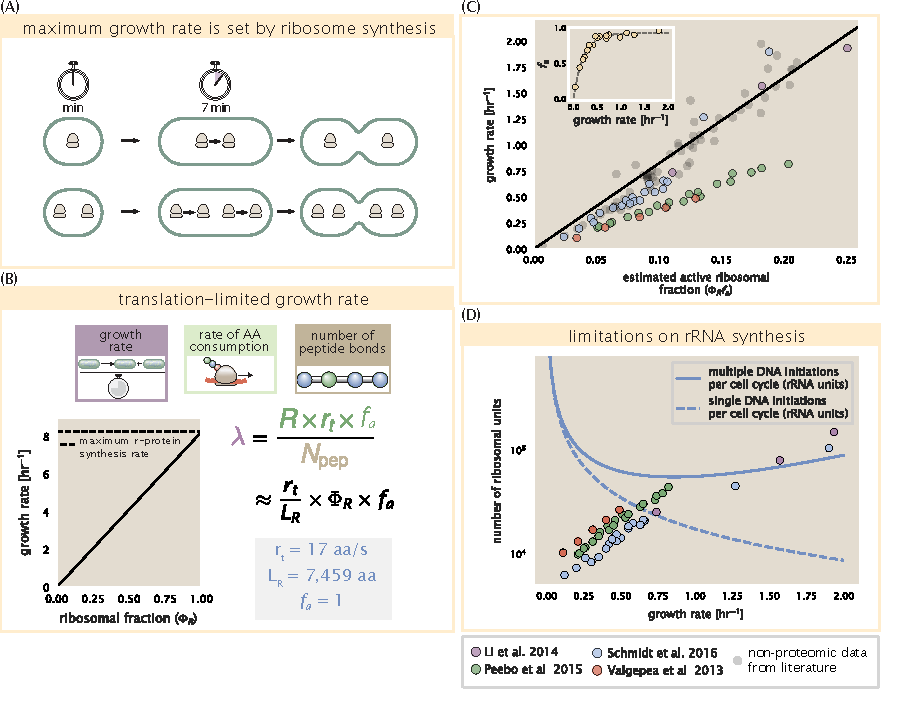
\includegraphics{main_figs/fig7_ribosome_as_limit.pdf}
        \caption{\textbf{Translation-limited growth rate.}  (A) An inherent
        maximum growth rate is set by the time to synthesize all ribosomal
        subunits. This growth rate is given by $r_t/ L_R$, where $r_t$ is
        the elongation rate and $L_R$ is the total number of amino acids
        that make up the entire ribosomal complex. This rate is independent
        of the number of ribosomes and instead is limited by the time required to
        double an individual ribosome. (B)
        Translation-limited growth as a function of the ribosomal fraction. The
        solid line is calculated for an elongation rate of 17 aa per second.
        The dashed line corresponds to the maximum rate of ribosomal protein
        (R-protein) synthesis considered in part (A).
        (C) Actively translating ribosomal fraction versus growth rate.
        The actively translating ribosomal fraction is calculated using the
        estimated values of $f_a$ from  \cite{dai2016} (shown in inset; see
        Appendix \nameref{sec:SI_f_a} for additional detail).
        (D) Maximum number of
        rRNA units that can be synthesized as a function of growth rate.
        Solid curve corresponding to the rRNA copy number is calculated by
        multipyling the number of rRNA operons by the estimated number of
        $\langle\text{\# ori}\rangle$ at each growth rate. The quantity
        $\langle\text{\# ori}\rangle$ was calculated using Equation 4 and
        the measurements from \cite{si2017} that are plotted in
        \FIG{translation_ecoli_partA}(A). The dashed line shows the maximal
        number of functional rRNA units produced from a single chromosomal
        initiation per cell cycle. }
        \label{fig:ribosome_limit}


        \figsupp[Comparison of $\Phi_R f_a$ with literature and estimation of $\langle$\# ori$\rangle$.]{(A) Actively translating ribosomal fraction versus growth rate.
        The actively translating ribosomal fraction is calculated using the
        estimated values of $f_a$ from  \cite{dai2016} (shown in inset; see
        Appendix \nameref{sec:SI_f_a} for additional detail). Additional measurements
        in addition to the proteomic measurements are based on measurements of cellular RNA to
        protein ratio, with $\Phi_R \approx$ the cellular RNA to
        protein ratio divided by 2.1 \citep{dai2016}. (B) Experimental measurements of
        the cell doubling time $\tau$ and cell cycle time $t_{cyc}$
         from Si \textit{et al.}
        (2017). Dashed line shows fit to the data, which were used to estimate
        $\langle$\# ori$\rangle$. $t_{cyc}$ was assumed to vary in proportion to
        $\tau$ for doubling times greater than 40 minutes, and reach a
        minimum value of 73 minutes. See Appendix
        \nameref{sec:SI_ori} for additional details exact estimation of rRNA copy number. Red data points correspond
        to measurements in strain MG1655, while light green points are for
        strain NCM3722.
        Schematic shows the expected increase in replication forks (or number of
        ori regions) as \textit{E. coli} cells grow faster. }{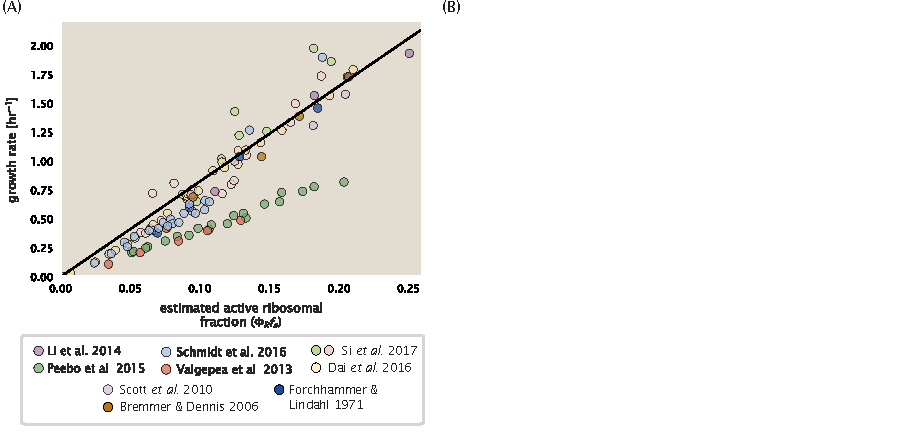
\includegraphics{main_figs/fig7_ribosome_as_limit_Supp.pdf}}\label{figsupp:ribosome_limit_supp}
        }
  \end{fullwidth}
\end{figure}

\subsection{rRNA Synthesis Presents a Potential Bottleneck during Rapid Growth}
\textit{E. coli} rarely exhibits growth rates above 2 hr$^{-1}$
\citep{bremer2008}, which is still well-below the synthesis rate of a single
ribosome, and below the growth rates reported for several other bacteria
\citep{roller2016}. Here we need to also consider ribosomal synthesis from the
perspective of limiting rRNA synthesis, which as we have found earlier, will depend on the
number of rRNA operons to transcribe rRNA.

Due to multiple rounds of chromosomal replication per cell doubling, the
effective number of rRNA operons increases with growth rate and will vary in
proportion to the average number of origins per cell, $\langle$\# ori$\rangle$.
This parameter is set by how often replication must be initiated per cell
doubling in order to maintain steady state growth, and quantified by
\begin{equation}
    \langle \text{\# ori} \rangle = 2^{\tau_{cyc} / \tau} = 2^{\tau_{cyc} \lambda / ln(2)}.
    \label{eq:Nori}
\end{equation}
Here, $t_{cyc}$ is the cell cycle time (referring to the time from replication
initiation to cell division), and $\tau$ is the cell doubling time.  We used the
experimental measurements of $\tau_{cyc}$ and  $\tau$ from \cite{si2017}
(\FIGSUPP[ribosome_limit]{ribosome_limit_supp}(B)) to calculate $\langle$\#
ori$\rangle$  with \EQ{Nori} as a function of growth rates. For growth rates
above about 0.5 hr$^{-1}$, $t_{cyc}$ is approximately constant at about 70
minutes, which means that $\langle$\# ori$\rangle$ will grow exponentially with
growth rate. Since the rRNA operons are predominantly located near to origin of
replication  (BNID: 100352, \cite{dennis2004}), we make the simplifying
assumption that that the number of rRNA operons  will be directly proportional
to $\langle$\# ori$\rangle$.

Returning to our rule-of-thumb of 1 functional rRNA unit per second per operon,
we estimate the maximum number of ribosomes that could be made as a function of
growth rate (\FIG{ribosome_limit}(C), blue curve). Although we expect this
estimate to drastically overestimate rRNA abundance at slower growth rates
($\lambda < 0.5\, \text{hr}^{-1}$), it provides a useful reference alongside the
proteomic measurements. For growth rates above about 1 hr$^{-1}$, we find that
cells will \texit{need} to transcribe rRNA near their maximal rate. As a counter
example, if \textit{E. coli} did not initiate multiple rounds of replication,
they would be unable to make enough rRNA for the observed number of ribosomes
(dashed blue curve in \FIG{ribosome_limit}(C)). The convergence between the
maximum rRNA production and measured ribosome copy number suggests rRNA
synthesis may begin to present a bottleneck at the fastest growth rates due to
the still-limited copies of rRNA genes.


% It is now well-documented that \textit{E. coli} cells add a constant volume per
% origin of replication, which is robust to a remarkable array of cellular
% perturbations \citep{si2017}.

% To consider
% this  in the context of the proteomic data, we used measurements of $\tau_{cyc}$
% and  $\tau$ from \cite{si2017} (\FIG{translation_ecoli_partA}(A)) to
% calculate $\langle$\# ori$\rangle$  with \EQ{Nori} at different growth
% rates. For ribosomal synthesis, we find an approximately linear correlation
% between ribosome copy number and $\langle$\# ori$\rangle$
% (\FIG{translation_ecoli_partA}(B)).
%
% For a constant cell cycle time, which is observed at growth rates above about
% 0.5 hr$^{-1}$ (\FIG{translation_ecoli_partA}(A), \citep{helmstetter1968}),
% \EQ{Nori} states that $\langle \text{\# ori} \rangle$ will need to increase
% exponentially with the growth rate.
